% !TEX encoding = UTF-8 Unicode
\documentclass[10pt,ngerman]{scrartcl}
\usepackage{url,bm,tikz,a4wide}
\usepackage[utf8]{inputenc}
\usepackage{booktabs}
\usepackage{amsmath,amssymb}
\usepackage[english]{babel}
\usepackage{graphicx,tikzsymbols} 
\usepackage{xcolor}
\usepackage[numbers]{natbib}
\usepackage{float}
\usepackage{gensymb}
\usepackage{pdfpages}
\usepackage{pdflscape}
\usepackage{hyperref}

\DeclareOldFontCommand{\bf}{\normalfont\bfseries}{\mathbf}

\usepackage{nicefrac,xfrac}

\renewcommand{\theenumi}{\alph{enumi})}
\renewcommand{\theenumii}{\Roman{enumii}}

\setcounter{secnumdepth}{-1}

\begin{document}

\begin{figure}[htbp]
\begin{minipage}[b]{0.50\linewidth}
\begin{Large}
	\textbf{Group Number:} 2\newline\newline
\end{Large}
\end{minipage}
\begin{minipage}[b]{0.50\linewidth}
\begin{flushright}
\begin{Huge}
\textbf{Physics}\\
\end{Huge}
\vspace{0.5cm}
\begin{large}
Winter term 2021/22
\end{large}
\end{flushright}
\end{minipage}
\end{figure}

\vspace{2cm}
\begin{huge}
\noindent

\textbf{Group Work}
\end{huge}

\section{1 Momentum and Force. Fields of Force}
\subsection{1.1 Momentum and Force. Fields of Force}
The so-called neutron stars have about the mass of our sun (ca. $2 \cdot 10^{30}kg$) and a typical diameter of about 20 km. Their mean mass density is roughly that of an atomic nucleus.
\begin{enumerate}
	\item How big is the mean mass density?
	\begin{align*}
		V_{Sphere} &= (\frac{4}{3}) \cdot \pi \cdot r^3\\
		p &= \frac{m}{V} = \frac{m}{(\frac{4}{3}) \cdot \pi \cdot r^3}\\
		p &= \frac{2 \cdot 10^{30}kg}{(\frac{4}{3}) \cdot \pi \cdot (10000m)^3} = 4.775 \cdot 10^{17} kg/m^3
	\end{align*}
	The mean mass of a neutron star is approximately $4.775 \cdot 10^{17} kg/m^3$\newline
	\item According to Newton's law of gravitation, how heavy would a piece of weight with the mass of 1kg be on the surface of a neutron star?
	\item How heavy would $1mm^3$ of neutron star matter be on earth and what diameter would an iron ball of the same mass have?
\end{enumerate}

\subsection{1.2 Coulomb interaction of two electrons}
Sketch correctly to scale the course of the magnitude of the force with which two electrons repel each other at distances of $0,5 \cdot 10^{-10}$m to $5,0 \cdot 10^{-10}$m according to Coulomb's law.
\begin{align*}
	[Q] &= As \\
	e &= 1.6022 * 10^{-19} As \\
	Q &= n * e \\
	Q_{1} &= Q_{2} = e = 1.6022 * 10^{-19} As \\
	\epsilon &= \epsilon_{0} * \epsilon_{r} \\
	\epsilon_{0} &= 8.854 * 10^{-12} \frac{As}{Vm} \\
	\epsilon_{r} &= 1 (\epsilon_{r} \text{ for vaccuum})\\
	\vec{F_{Q1}} &= \frac{1}{4 * \pi * \epsilon } * \frac{Q_{1}*Q_{2}}{r^{2}} * \frac{\vec{r}_{12}}{|\vec{r}_{12}|} = -\vec{F_{Q2}}
\end{align*}
See sketch on next page and calculation of data points in appendix \hyperref[sec:data-table-a2]{3.1 Data table 1.2 (A2)}

\begin{landscape}
 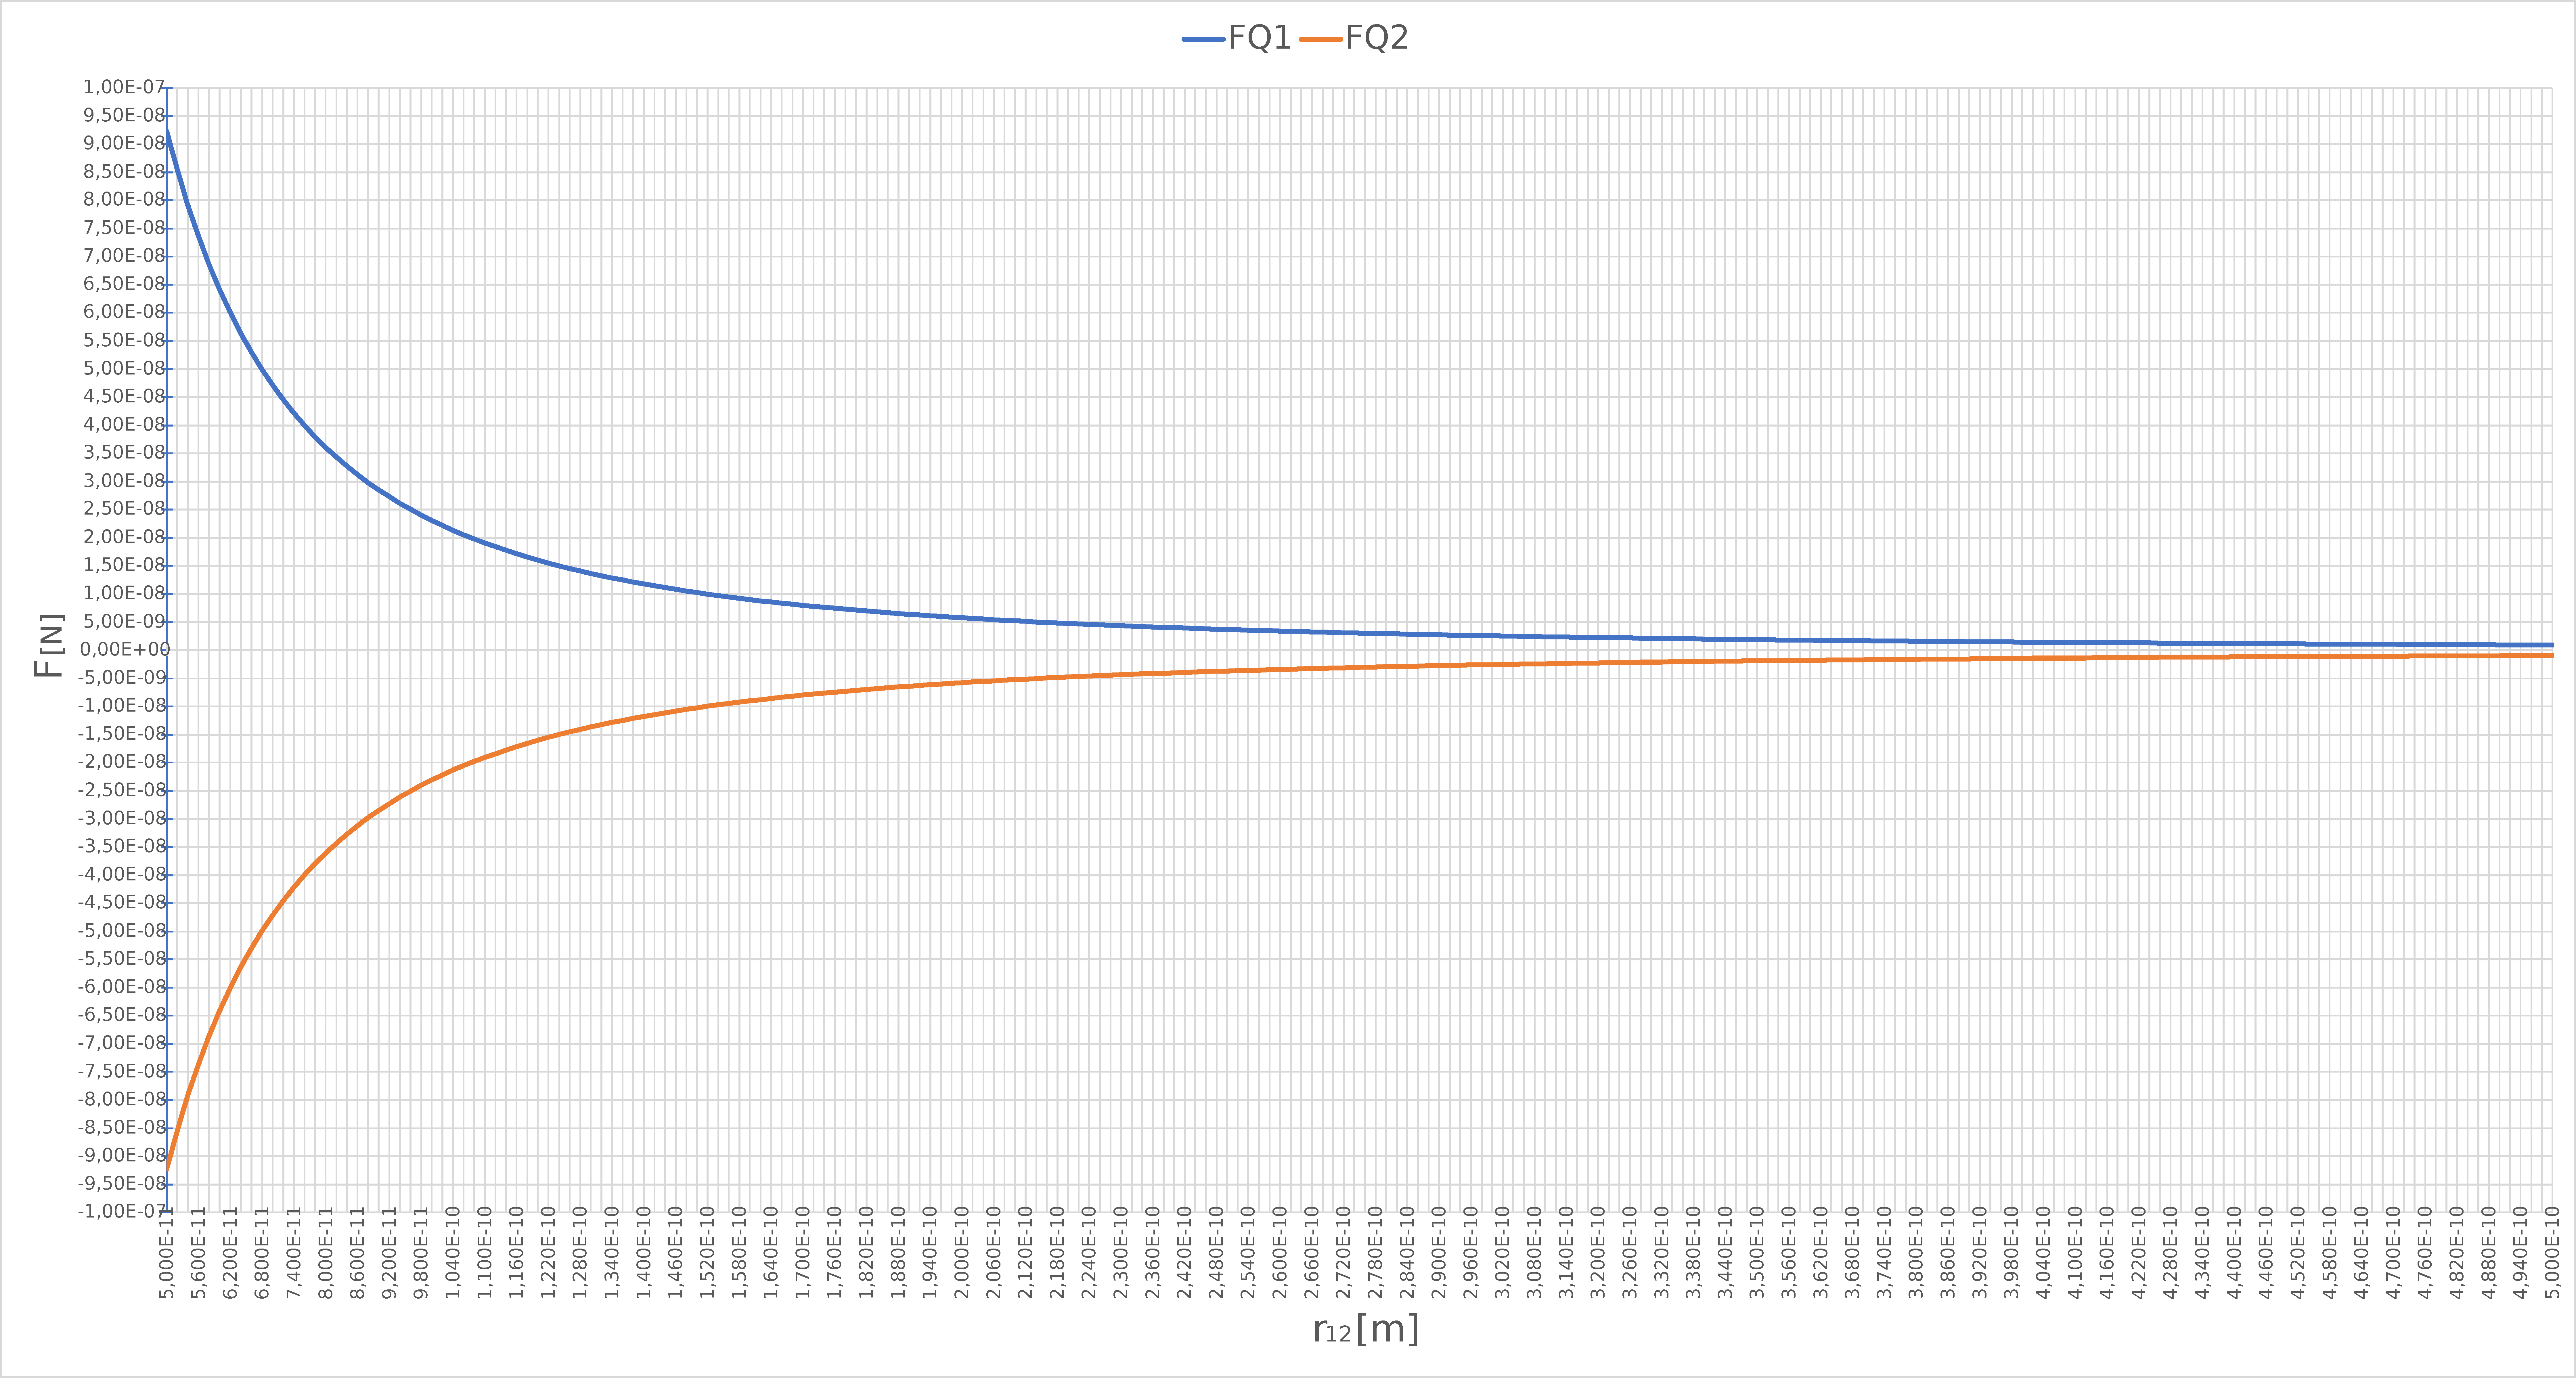
\includepdf[pages={-},angle=90]{force_a2.pdf}
\end{landscape}

\newpage
\section{2 Work and Power. Energy. Heat and Temperature}
\section{2.1 train set}
For example, the electric drive of a train set consumes the power shown in the figure below during a operational cycle (1 MW = 106 W).

\begin{enumerate}
	\item What is the total electrical energy consumed during this operational cycle?
	\begin{align}
		P_{1} &= \frac{7MW\cdot 120s}{2} = 420MWs = 420MJ\\
		P_{2} &= 2 MW * 600s = 1200 MW = 1.2 GJ\\
		P_{3} &= \frac{-7MW * 60s}{2} = -240 MW\\
		P_{total} &= P_{1} + P_{2} + P_{3} = 420MJ + 1.2 GJ - 240 MJ = 1.38 GJ
	\end{align}
	\item What is the mean power consumed?
	\begin{align}
        P_{mean} = \frac{P_{total}}{\Delta t} = \frac{1.38 GJ}{\Delta t_{1} +\Delta t_{2} +\Delta t_{3} +\Delta t_{4}}
		= \frac{1.38GWs}{120s + 600s + 60s + 60s} = 1.643MW
    \end{align}
\end{enumerate}

\begin{figure}[H]
	\centering
	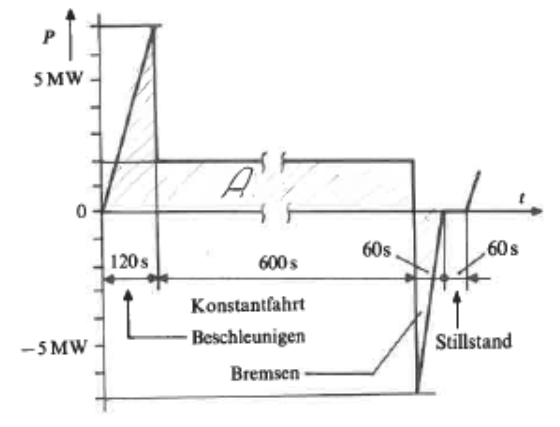
\includegraphics[scale=0.5]{group_work_1.png}
\end{figure}

\section{2.2 crash test facility}
In a crash test facility, a vehicle including cuts m = 900 kg is accelerated uniformly via an electric linear motor through a distance s = 20 m with a constant force F = 5 kN.
\begin{enumerate}
	\item How big is the necessary electrical energy in kWh if all losses are neglected?
	\item How big is the final speed achieved? During the subsequent impact process, the vehicle is brought to a standstill within a distance of s = 80 cm.
	\item What is the mean force that acts on a fictitious seated occupant, m1 = 80 kg?
\end{enumerate}

\section{2.3 Connected load of a flow heater}
Suppose you want to design an electric water heater without a storage tank that heats a water flow of 0,1 l/s from 10 °C to 60 °C. 
What is the minimum required electrical connection power? (specific heat capacity of water c = 4,19 kJ/(kgK)).
\newline
\begin{flalign*}
	&T_{in} = 10\degree C&\\
	&T_{out} = 60\degree C&\\
	&\Delta T = 50^{\degree}C = 50K&\\
	&\text{water flow} = 0.1l/s&\\
	&m = 0.1kg&\\
	&\text{specific heat capacity of water c} = 4.19kJ/(kgK)&\\
	&\text{total energy to heat up 0.1l water } \Delta Q = c \cdot m \cdot \Delta T&\\
	&\text{minimum required electrical connection power } [W] = kWh&
\end{flalign*}
Required energy to heat up 0.1 kg water from $10\degree$C to $60\degree$C
\begin{align*}
	\left[\Delta Q\right] = K \cdot kg \cdot \frac{kJ}{kg \cdot K} = kJ\\
	\Delta Q = 50 \cdot 0.1 \cdot 4.19 = 20.95kJ
\end{align*}
Required connection power to heat up 0.1l/s water from $10\degree$C to $60\degree$C\newline
$\left[P\right] = W$\newline
$P = \frac{E}{t_{s}}$ ($t_{s}$ $\rightarrow$ time period in seconds $\rightarrow$ in this case one second because of heating up the specific amount of water every second)
\begin{align*}
	P = \frac{20950}{1} = 20950W = 20.95kW
\end{align*}

\newpage
\section{3.0 Appendix}
\subsection{3.1 Data table 1.2 (A2)}
\label{sec:data-table-a2}
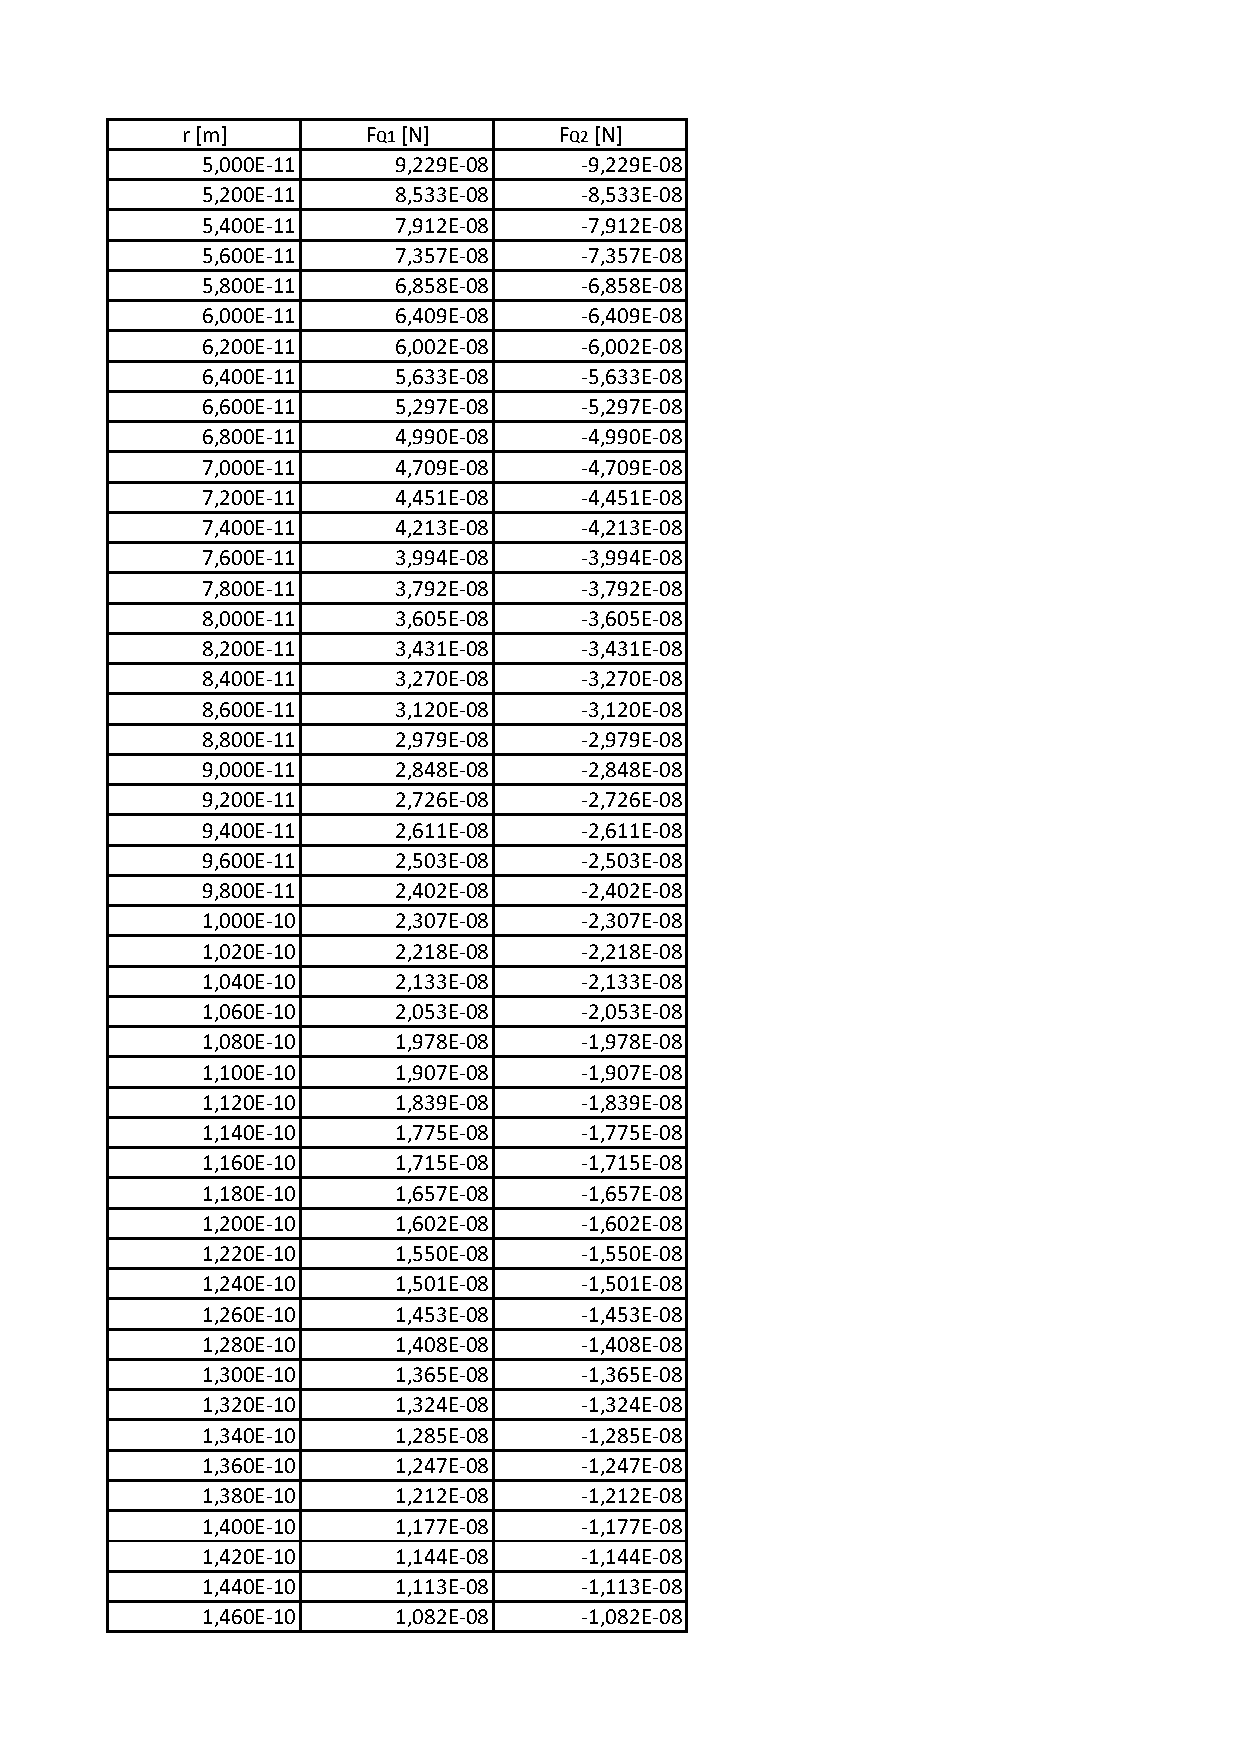
\includepdf[pages=-]{a2_table.pdf}

\end{document}